\documentclass[12pt,twoside]{article}

\usepackage{lapsiohje}

\usepackage[ampersand]{easylist}
\usepackage[finnish]{babel}
\usepackage[utf8]{inputenc}
\usepackage{sectsty}
\usepackage{titlesec}
\usepackage{enumitem}
\usepackage{amssymb}
\usepackage{fancyhdr}
\usepackage{graphicx}
\usepackage{hyperref}


\usepackage{sidecap}
\usepackage[font=sf]{caption}
\sidecaptionvpos{figure}{t}

\sectionfont{\fontfamily{lmss}\fontsize{35}{35}\selectfont}
\subsectionfont{\fontsize{25}{40}\fontfamily{lmss}\selectfont}
\titlespacing*{\section}{3em}{0em}{2em}
\titlespacing*{\subsection}{1.5em}{1em}{1em}

\usepackage{geometry}
 \geometry{
 a4paper,
 total={170mm,240mm},
 left=20mm,
 top=25mm,
 footskip=18mm
 }

\fontfamily{lmss}\selectfont 
\pagestyle{fancy}
\fancyhf{}
\renewcommand{\headrulewidth}{0pt}
\fancyhead[LE,RO]{\thepage}
\lfoot{\fontfamily{lmss}\selectfont Creative Commons BY-NC-SA}
\rfoot{\fontfamily{lmss}\selectfont Alkuperäinen tekijä (\the\year) Anni Järvenpää}

\setitemize{topsep=0pt,parsep=10pt}


% tästä alkaa varsinainen ohje, kaikki yläpuolella säätää fontteja, marginaaleja yms. mitä ei lähtökohtaisesti tarvitse säätää uutta ohjetta tehdessä
\begin{document}
\fontfamily{lmss}\selectfont
\section*{Pelin nimi}

\begin{SCfigure}[][h]
  \centering
  \captionsetup{labelformat=empty}
  \caption{Lyhyt kuvaus pelistä, mitä siinä tehdään ja mihin pyritään. \href{https://google.fi}{Linkki mallipeliin}, tekijän nimi ja pelin nimi näkyviin että tulosteenkin perusteella on mahdollista löytää.}
  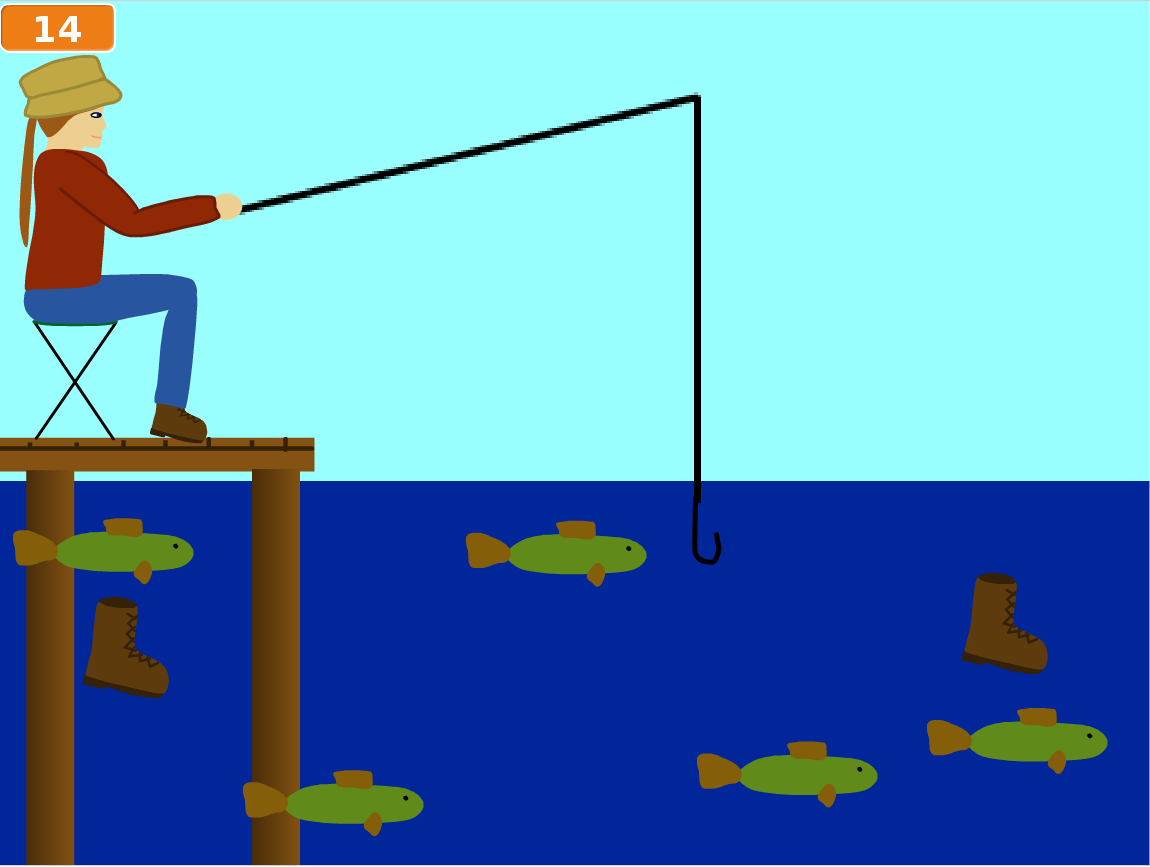
\includegraphics[width=0.7\textwidth]{kuvat/esimerkki.png}
\end{SCfigure}

\begin{vaihetaso1}
	\item Ensimmäinen ohje.
	
	\begin{vaihetaso2}
		\item Yhden lauseen kuvaus
		\item Tällä on alakohta
		
		\begin{vaihetaso3}
			\item Turhan syvä alakohta
		\end{vaihetaso3}
		\item Pitkähkö kuvaus siitä, mitä nyt pitää tehdä. Monimutkaiset ohjelmat ovat monimutkaisia. Onneksi lapset ovat fiksuja.
	\end{vaihetaso2}
	\item Toinen vaihe
	
	\begin{vaihetaso2}
		\item Laatikoita pukkaa
		\item Tällä on alakohta
		\item Lorem ipsum
	\end{vaihetaso2}
	\item Kolmas vaihe
	\item Neljäs vaihe
\end{vaihetaso1}

\subsection*{Esimerkkejä värien käytöistä}
\begin{vaihetaso1}
	\item \textcolor{liike}{Liikunta} on tärkeämpää kuin \textcolor{ulkonako}{ulkonäkö}. 
	
	\begin{vaihetaso2}
		\item Välillä voi käyttää \textcolor{aani}{ääntä}. Kirjoitan vain pitkän tekstin että tämä menee kahdelle riville.
		\item Oispa \textcolor{muuttujat}{muuttujia}. Tahtoisin tämänkin vaativan ainakin kaksi riviä.
		
		\begin{vaihetaso3}
			\item Muita vaihtoehtoja ovat \textcolor{tapahtumat}{tapahtumat}, \textcolor{ohjaus}{ohjaus} ja \textcolor{tuntoaisti}{tuntoaisti}.
		\end{vaihetaso3}
	\end{vaihetaso2}
	
	\item \textcolor{lohkot}{Lohkot} \textcolor{toiminnot}{toimii}.
	\item \textcolor{laajennus}{Kynä} on uudessa Scratchissa laajennus eli samalla värillä kuin esimerkiksi \textcolor{laajennus}{musiikki-} ja \textcolor{laajennus}{käännöspalikat}.
	\item Myös vanhan scratchin värejä voi tarvittaessa käyttää. Ne on merkattu numerolla 2 nimen lopussa, esim \textcolor{lohkot2}{vanhat lohkot}.
\end{vaihetaso1}

\subsection*{Ikoneita}
\begin{vaihetaso1}
	\item Scratch 3.0:
	
	\begin{vaihetaso2}
		\item Pelin voi käynnistää $\lippu$ tai pysäyttää $\pysayta$.
		\item Valitse hahmo -valikosta $\hahmovalikko$ löytyy kaikenlaista, voit esimerkiksi lähettää kuvan koneelta $\lataa$, valita satunnaisen kuvan $\yllata$, piirtää itse $\piirra$ tai valita itse valmiista hahmoista $\valitse$.
		\item Myös taustavalikko $\taustavalikko$ on kiinnostava, siellä on samat vaihtoehdot.	
	\end{vaihetaso2}
	\item Wanha scratch (merkattu kirjaimella ''W'' nimen jälkeen):
	
	\begin{vaihetaso2}
		\item Grafiikoita voi piirtää $\piirraW$ tai valita valmiina $\valitseW$. Vihreästä lipusta $\lippuW$ starttaa.
		\item Yläpalkissa on myös namiskoja, esim $\kopioiW$ kopiointi, $\poistaW$ poisto, $\kasvataW$ kasvatus ja $\pienennaW$ pienennys.
		\item Hahmojen kiertotyyliksi voi asettaa $\jokasuuntaanW$, $\vasenoikeaW$ tai $\alakierraW$.
	\end{vaihetaso2}
\end{vaihetaso1}


% halutessaan voi alemman %-merkin poistamalla pakottaa laajennusideat omalle sivulleen
%\newpage
\subsection*{Laajennusideoita}
\begin{itemize}
	\item[-] Muita hauskoja juttuja, joita peliin voisi halutessaan toteuttaa
	\item[-] Voi olla myös alakohtia:
	
	\begin{itemize}
		\item[-] Ensimmäinen alakohta
		\item[-] Toinen alakohta
		\item[-] Kolmas alakohta
	\end{itemize} 
	
	\item[-] Vielä tavallinen idea perään
\end{itemize}

\end{document}